\documentclass[11pt]{article} 

\usepackage{fullpage}
\usepackage{fancybox}
%\usepackage{oz}
\usepackage{multicol}
\usepackage{ifthen}
\usepackage{version}
\usepackage{url}
\usepackage{amsfonts}
\usepackage{amsmath}
\usepackage{graphicx}
\usepackage{enumerate}
\usepackage{booktabs}
\usepackage{hyperref}

\newlength{\tab}
\setlength{\tab}{1em}
\setlength{\parindent}{0pt}
\setlength{\parskip}{6pt}
\setlength{\evensidemargin}{0.0cm}
\setlength{\oddsidemargin}{0.0cm}
\setlength{\textwidth}{16cm}
%  \setlength{\headsep}{0cm}
\setlength{\headheight}{0cm}
\setlength{\topmargin}{0cm}
\setlength{\textheight}{23cm}
\setlength{\itemsep}{0pt}
\setlength{\topsep}{0pt}


\definecolor{javared}{rgb}{0.6,0,0} % for strings
\definecolor{javagreen}{rgb}{0.25,0.5,0.35} % comments
\definecolor{javapurple}{rgb}{0.5,0,0.35} % keywords
\definecolor{javadocblue}{rgb}{0.25,0.35,0.75} % javadoc
\definecolor{javabackground}{rgb}{0.9,0.9,0.9}
\definecolor{javablack}{rgb}{0,0,0}

\lstset{language=Ada,
  backgroundcolor=\color{javabackground},
  basicstyle=\ttfamily\fontsize{10}{12}\selectfont,
  keywordstyle=\color{javablack}\bfseries,
  aboveskip={1.5\baselineskip},
  stringstyle=\color{javared},
  commentstyle=\color{javagreen},
  morecomment=[s][\color{javadocblue}]{/**}{*/},
  numbers=left,
  numberstyle=\tiny\color{black},
  frame=single,
  numbersep=10pt,
  stepnumber=1,
  tabsize=8,
  xleftmargin=0ex,
  xrightmargin=0ex,
  showspaces=false,
  showstringspaces=false,
  aboveskip=0.5ex
}


\usepackage[textsize=scriptsize,textwidth=1cm]{todonotes}
\newcommand{\tm}[1]{\todo[inline,color=yellow]{#1}}
%=======================================================================
%      New Environments
%
\newtheorem{definition}{Definition}
\newtheorem{theorem}[definition]{Theorem}
\newtheorem{proposition}[definition]{Proposition}
\newtheorem{lemma}[definition]{Lemma}
\newtheorem{remark}[definition]{Remark}
\newtheorem{exercise}[definition]{Exercise}
\newtheorem{example}[definition]{Example}

\newenvironment{omitable}[1]{}

%----------------------------------------------------------------------
%    The Document
%

\newcommand{\assignmenttitle}[2]{
\begin{center}
\textbf{\sc The University of Melbourne}\\[0.5ex]
\textbf{\sc SWEN90010: High Integrity Software Engineering}\\[1ex]
\textbf{\large Assignment {#1}}\\[1ex]
%\textbf{\sc Second Semester, 2014}\\[1ex]
\textbf{\sc Due Date: #2}
\end{center}
}


\newcommand{\solutionstitle}[2]{
\mbox{}\\
%\vspace{10ex}
\begin{center}n
\textbf{\sc The University of Melbourne}\\[0.5ex]
\textbf{\sc SWEN90010: High Integrity Software Engineering}\\[1ex]
\textbf{\large Assignment {#1} Solutions}\\[1ex]
%\textbf{\sc Second Semester, 2014}\\[1ex]
\textbf{\sc Due Date: #2}
\end{center}
\vspace{5ex}
}


\begin{document}

\assignmenttitle{1}{11:59pm, Sunday 22 March, 2015}

\section{Introduction}

This assignment is worth 10\% of your total mark.

The aim of this assignment is to provide you with an opportunity to implement a simplified safety- and security-critical system in Ada. Doing so will help to explore the properties of Ada, and how they relate to safe programming.

\textbf{Tip:} Perhaps the most difficult part of this assignment is getting your head around the system itself, and the packages already supplied. Be sure to download the provided code early, and to understand the example scenario and how its uses the interfaces of the supplied packages.


\section{System overview}

The system to be produced as part of the assignment is part of a \emph{simulation} of a real medical device called an \emph{implantable cardioverter-defibrillator} (ICD).

In ICD is a battery-powered device implanted into patients who are at risk of cardiac arrest (heart attack) due to ventricular fibrillation and ventricular tachycardia. The device is battery powered, and monitors electrical impulses from the right ventricle of patient's heart, delivering powerful electric pulses if an anomaly is detected. The device is similar to a pacemaker.

Figure~\ref{fig:icd}\footnote{Image from Wikimedia Commons} shows an illustration of an ICD as it would be implanted in a person. The small box labelled \emph{Implantable Cardioverter-Defibrillator} is where the critical decision making occurs. It consists of several components, however in this project, we will consider only three: (1) a heart rate monitor; (2) a decision-making system (software controlled); and (3) an impulse generator.

\begin{figure}[!h]
 \centering
 \includegraphics[scale=0.27]{./figs/ICD_InsideLeads}
 \caption{Implantable cardioverter-defibrillator (ICD)}
 \label{fig:icd}
\end{figure}

Figure~\ref{fig:icd-loop} shows the closed-loop control for these three components. From this figure, one can see that the patient's heart rate is measured using the heart-rate monitor in the device. The ICD software must determine whether the heart  is behaving normally, or whether a critical event, such as ventricular fibrillation, is occurring. If it has determined this, it much decide whether to deliver a pulse into the heart using the impulse generator, and if so, how much, thereby directly influencing the beat of the heart. This loop continues unbounded.

\begin{figure}[!h]
 \centering
 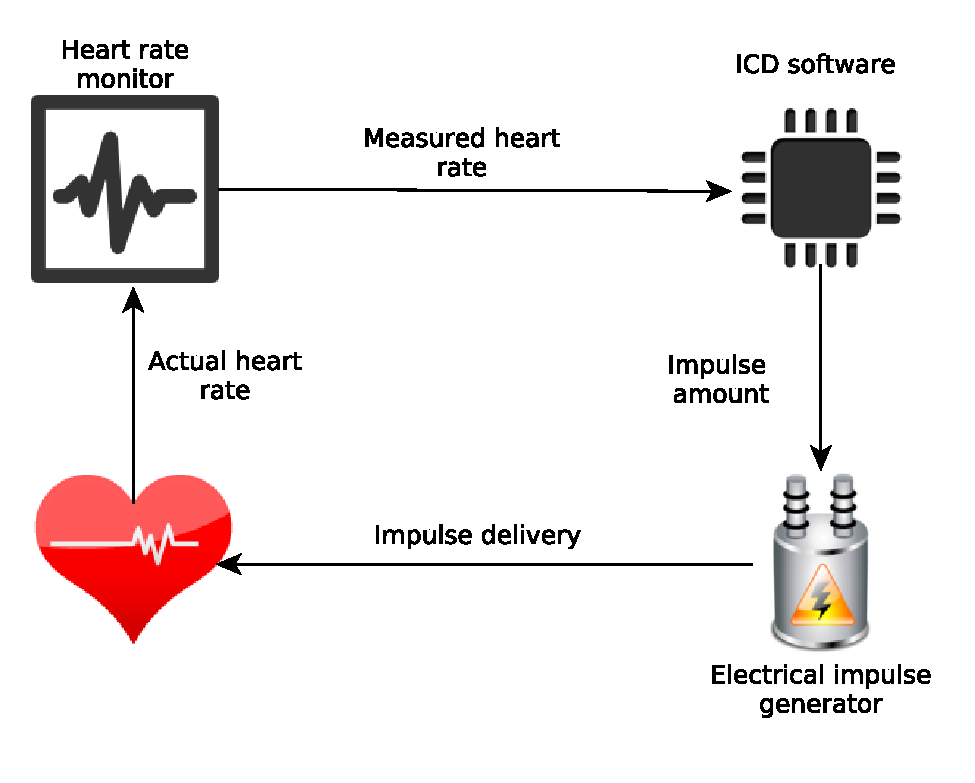
\includegraphics[scale=0.6]{./figs/icd-loop}
 \caption{ICD closed loop.}
 \label{fig:icd-loop}
\end{figure}

Note the difference between the signal and the actual in this figure. That is, there is an actual heart rate, and a \emph{measured} heart rate, which may be incorrect due to malfunction or low accuracy of the monitor. Similarly, the impulse amount specified to the impulse generator may not be what the generator ultimately delivers, should the generator have problems.

While the system is specified as a closed loop, ICDs can also be interacted with via wireless data connections, allowing settings to be changed.

The safety-critical aspects of this system are clear: if the impulse delivered to the patient is wrong, it can cause significant health risks, including, at worst, death. 

\section{User requirements}
\label{sec:user-requirements}

\subsection{Definitions}

\begin{enumerate}[~~\bf{D}1]

 \item \emph{bpm} (\emph{beats per minute}): a unit of measuring heart rate.

 \item \emph{Tachycardia}: A fast heart rate, typically defined as above 100 bpm at rest. A more complete definition: ``A rapid life-threatening rhythm originating from the lower chambers of the heart. The rapid rate prevents the heart from filling adequately with blood, and less blood is able to pump through the body''\footnote{\url{http://www.webmd.com/heart-disease/heart-disease-glossary-terms}}.

% \item \emph{Bradycardia}: A slow heart rate, typically defined as below 50 bpm at rest.

 \item \emph{Ventricle fibrillation}: ``An erratic, disorganised firing of impulses from the ventricles. The ventricles quiver and are unable to contract or pump blood to the body''$^2$. Typically leads to cardiac arrest.

 \item \emph{Joules}: The unit of energy used for delivering electrical impulses. Formally defined as the amount of energy required to apply a force of one Newton through one metre.

 \item \emph{ds (decisecond)}: One tenth of a second.

\end{enumerate}

\subsection{Roles}

There are three roles that take part in this system:

\begin{enumerate}

 \item \emph{Patient}: A person who has an ICD implanted into their chest.

 \item \emph{Cardiologist}: A medical doctor specialising in cardiology, who treats patients with an implanted ICD. A cardiologist is able to perform certain actions on an implanted ICD, such as reading data and changing settings.

 \item \emph{Clinical Assistant}: A medically-trained person who supports treatment of a patient with an implanted ICD. A clinical assistant is able to perform certain actions on an implanted ICD, such as reading data.

\end{enumerate}
Each Patient may have some particular cardiologist(s) or clinical assistant(s) assigned to care for them.

\subsection{Modes}

The system operates in one of two modes: \emph{off} and \emph{on}:

\begin{enumerate}[~~\bf{R1}.1]

  \item \emph{Off}: In the \emph{off} mode, the closed-loop functionality of the monitor is off to allow medical personnel to change settings on the device. 
%In this mode, no impulse is delivered  to the patient.

  \item \emph{On}: In the \emph{on} mode, the closed-loop functionality of the monitor is on, meaning that impulses may be delivered to the patient, and settings cannot be changed.

  \item An authorised Cardiologist or Clinical Assistant can switch between the modes. 

 % Precondition for switching.

  \item The initial mode is \emph{off}.

\end{enumerate}

\subsection{Off mode}
\label{sec:spec:off-mode}

The system must support the following requirements for the off mode:

\begin{enumerate}[~~\bf{R2}.1]

  \item In the off mode, the heart rate monitor and impulse generator must be switched off at all times.

 \item The patient must receive no electric impulse.

 \item An authorised Cardiologist or Clinical Assistant can read the settings; that is, the upper bound for tachycardia, and number of joules to deliver, etc.

 %System invariant: mode = off => impulse = 0.

% \item A medic can increase or decrease the lower bound for bradycardia.

 \item A Cardiologist can increase or decrease the upper bound for tachycardia.

 \item A Cardiologist can increase or decrease the number of joules delivered for a ventricle fibrillation.

% \item The initial lower bound for bradycardia when the system starts is 50 bpm.

 \item The initial upper bound for tachycardia when the system starts is 100 bpm.

 \item The initial number of joules to deliver in the case of a ventricle fibrillation is 30.

\end{enumerate}


\subsection{On mode}
\label{sec:spec:on-mode}

The system must support the following requirements for the on mode:

\begin{enumerate}[~~\bf{R3}.1]

% \item If a bradycardia is detected (the heart rate is under the specified lower bound), the impulse generator must deliver ten (10) signals at two (2) joules at the rate of 10bpm above the specified lower bound\footnote{Each signal makes the heart contract.}.

%   For example, if a bradycardia is detected and the specified lower bound is 50bpm, then the impulse generator should send 10 $\times$ 2 joule signals at 60bpm.

 \item If a tachycardia is detected (the heart rate is above the specified upper bound), the impulse generator must deliver ten (10) signals at two (2) joules at the rate of 15bpm \emph{above} the current heart rate.

  For example, if a tachycardia is detected and current heart rate is 110bpm, the impulse generator must deliver 10 $\times$ 2 joule signals at 125bpm.

 NOTE: the treatment for tachycardia is to \emph{increase} the heart rate. The shocks are designed to short-circuit the ventricular rhythms, attempting to disrupt the rhythm and halt the tachycardia.

 \item If a ventricle fibrillation is detected, the impulse generator must deliver one (1) single shock at the specified number of joules. See Section~\ref{sec:vf} for a definition of ventricle fibrillation.

 \item If no tachycardia or ventricle fibrillation is detected, the impulse generator should deliver no signal (zero joules).

\end{enumerate}

The system must supporting the following requirements in all modes:

\begin{enumerate}[~~\bf{R3}.4]

 \item An authorised Patient, Cardiologist, or Clinical Assistant can read the last 50 impulses that have been delivered, and the time they were delivered (where ``time'' is just the clock tick).

\end{enumerate}


\subsection{Impulse generator}

The system must support the following requirements for regarding the impulse generator:

\begin{enumerate}

 \item The impulse generator can be switched on or off.

\end{enumerate}

\paragraph{Constraints} The impulse generator has the following constraints/properties:

\begin{enumerate}

 \item The maximum number of joules the pump is able to administer is 45.

\end{enumerate}

\subsection{Heart rate monitor}

The system must support the following requirements for regarding the heart rate monitor:

\begin{enumerate}

 \item The heart rate monitor can be switched on or off.

\end{enumerate}

The heart rate monitor has the following constraints/properties:

\begin{enumerate}

 \item To simplify the assignment, the heart rate monitor provides  a heart rate in \emph{beats per minute} (bpm) every decisecond, rather than a wave form, as is common for real heart rate monitors. 

 This reading is based on the time between the \emph{previous two beats of the heart}.
% A safety hazard here if the heart flutters.

\end{enumerate}


\subsection{Detecting ventricle fibrillation}
\label{sec:vf}

Detecting ventricle fibrillation is a non-trivial task, and there are many algorithms available for this -- most work on wave patterns, which is far beyond the scope of this subject.

In this assignment, we will use just a rough approximation. A heart is defined to be in ventricle fibrillation if and only if: the average change in heart rate per reading over the previous six readings, is greater than or equal to 10 bpms. That is:
%
\[
\frac{\Sigma_{t=now-6}^{now}\ |(bpm(t) - bpm(t-1))|} {6} \geq 10
\]


\noindent in which $now$ is the most recent tick, and $bpm(t)$ returns the heart rate at time $t$.

\section{Existing packages}
\label{sec:existing-packages}

The following packages are available for download from the LMS. 
The first three simulate the heart, heart rate monitor, and impulse generator respectively:

\begin{enumerate}

 \item \texttt{Heart}: A (very crude) simulation of a patient's heart. A heart has heart rate, which can be affected electric impulses. The patient's heart rate changes over time, even if no impulse is sent from the generator.

 \item \texttt{ImpulseGenerator}: A simulation of an impulse generator. The generator is connected to a patient's heart, receives a target number of joules, and shocks the patient's heart with this amount.

 \item \texttt{HRM}: A simulation of a heart rate monitor. The monitor is connected to the patient's heart, can monitor the heart rate, and reports the current heart rate; if it could detect one. The monitor has a small error margin in its measures, meaning it is not completely accurate.

 \item \texttt{RandomNumber}: A package used to generate some random values for simulation purposes. You do not need to use this directly as part of your submission.

 \item \texttt{Measures}: A package containing the Ada types used to represent beats per minute (BPM) and joules.

 \item \texttt{ManualOperationExample}: A procedure containing an example simulating a scenario in which the various components are used, but not in closed-loop mode.

\end{enumerate}

Note that the first three of these each contain a procedure called \texttt{Tick}, which is used to simulate a one decisecond passage of time. So, when a shock is delivered to a patient's heart, the heart's \texttt{Tick} procedure must be called to simulate the delivery of that shock.

\section{Your tasks}

The tasks for the assignment are listed below:

\begin{enumerate}

 \item Implement an Ada package called \texttt{ICD}, which implements the functionality to provide the necessary calculations of the impulse to be delivered based on the measured heart rate.

 \textbf{Note}: Your solution should be more general than simply adjusting the impulse for the single heart that is implemented in the \texttt{Heart} package. That is, it should support hearts with different behaviour.

 \item Implement an Ada package called \texttt{ClosedLoop} that encapsulates the \texttt{ICD}, \texttt{Heart}, \texttt{HRM}, and \texttt{ImpulseGenerator} packages to fulfil the behaviour of an ICD device. The package interface should offer at least the following:

  \begin{enumerate}

    \item Adding authorised users.

    \item Switching between modes.

    \item Turning the heart rate monitor and impulse generator on/off.

    \item Changing the settings; e.g.\ the lower bound.

    \item Reading settings and the last 50 shocks.

    \item ``Ticking'' the clock one decisecond, which simply ticks all other entities in the system (ICD, Heart, HRM, and ImpulseGenerator).
  \end{enumerate}

  The last of these is for the purpose of stepping through a simulation. The remainder are all functions/procedures that can be exported directly to any user interface code. 

 \textbf{Note:} You do \emph{not} have to implement a user interface.

  The functions should use the packages outlined in Section~\ref{sec:existing-packages} to implement the behaviour of the heart, impulse generator, and monitor respectively. 

 \item A procedure called \texttt{ClosedLoopExample}, which implements a scenario showing how to use your \texttt{ClosedLoop} package, similar to that in the procedure \texttt{ManualOperationExample}. At a minimum, this must demonstrate switching from off mode to on mode, and then looping through the on mode for at least 100 ticks.

\end{enumerate}

You are encouraged to modify the code for the purpose of testing etc., however, we will use our own implementations of \texttt{Heart}, \texttt{ImpulseGenerator}, and \texttt{HRM} to run tests as part of the assessment.

\section{Criteria}

\begin{center}
\begin{tabular}{lp{10cm}l}
\toprule
 {\bf Criterion} & {\bf Description} & {\bf Marks}\\
\midrule
  Design & The design of the system is of high quality. The correct components have been included, the design is loosely coupled, and suitable information hiding strategies have been used. & 2 marks\\[2mm]
  Correctness & The implementation behaves correctly with respect to the user requirements. The automated mode detects anomalies correctly and acts on them appropriately.  & 2 marks\\[2mm]
  Completeness & The implementation is complete. All components have been implemented and all user requirements have been addressed. & 1 marks\\[2mm]
  Clarity & The design and implementation are clear and succinct. & 1 marks\\[2mm]
  Code formatting & The implementation adheres to the code format rules (Appendix~\ref{app:code-format-rules}). & 2 marks\\[2mm]
  Tests & The implementation passes our tests. & 2 marks\\[1mm]
\midrule
  Total && 10 marks\\
\bottomrule
\end{tabular}
\end{center}

\section{Submission}

Create a zip file called  \emph{your\_username}\texttt{.zip} or \emph{your\_username}\texttt{.tgz}. The file should contain your code for the \emph{complete} ICD system, including code provided by subject staff.

Submit the zip file to the LMS.

\section{Academic Misconduct}

The University misconduct policy applies to this assignment. Students are encouraged to discuss the assignment topic, but all submitted work must represent the individual's understanding.

The subject staff take plagiarism very seriously. In the past, we have successfully prosecuted several students that have breached the university policy. Often this results in receiving 0 marks for the assessment, and in some cases, has resulted in failure of the subject.

\pagebreak

\appendix

\section{Code format rules}
\label{app:code-format-rules}

The layout of code has a strong influence on its readability. Readability is an important characteristic of high integrity software. As such, you are expected to have well-formatted code. 

A code formatting style guide is available at \url{http://en.wikibooks.org/wiki/Ada_Style_Guide/Source_Code_Presentation}. You are free to adopt any guide you wish, or to use your own. However, the following your implementation must adhere to at least the following simple code format rules:

\begin{itemize}

\item Every Ada package must contain a comment at the top of the specification file indicating its purpose.

\item Every function or procedure must contain a comment at the beginning explaining its behaviour. In particular, any assumptions should be clearly stated.

\item Constants and variables must be documented.

\item Variable names must be meaningful.

\item Significant blocks of code must be commented.

However, not every statement in a program needs to be commented. Just as you can write too few comments, it is possible to write too many comments.

\item Program blocks appearing in if-statements, while-loops, etc. must be indented consistently. They can be indented using tabs or spaces, and can be indented any reasonable number of spaces (three is default for Ada), as long as it is done consistently.

\item Lines must be no longer than 80 characters. You can use the Unix command ``\texttt{wc -L *.ad*}'' to check the maximum length line in your Ada source files.

\end{itemize} 

% LocalWords:  wc adb

\end{document}

% LocalWords:  hypotension patient's intravascular hypoperfusion  bpm
% LocalWords:  HRM ICD  RandomFloat ManualOperationExample lp ICDs ds
% LocalWords:  ClosedLoop AutomatedModeExample cardioverter Wikimedia
% LocalWords:  decisecond ImpulseGenerator RandomNumber MVC bpms LMS
% LocalWords:  ClosedLoopExample
